%%%%%%%%%%%%%%%%%%%%%%%%%%%%%%%%%%%%%%%%%%%%%%%%%%%%%%%%%%%%%%%%%
% Tese de Doutorado / Dept Fisica, CFM, UFSC                    %
% Andre@UFSC - 2014                                             %
%%%%%%%%%%%%%%%%%%%%%%%%%%%%%%%%%%%%%%%%%%%%%%%%%%%%%%%%%%%%%%%%%

%:::::::::::::::::::::::::::::::::::::::::::::::::::::::::::::::%
%                                                               %
%                          Capítulo 7                           %
%                                                               %
%:::::::::::::::::::::::::::::::::::::::::::::::::::::::::::::::%

%***************************************************************%
%                                                               %
%               Estudo das populações estelares                 %
%                                                               %
%***************************************************************%

\chapter{Estudo das populações estelares}
\label{sec:pop}

%***************************************************************%
%                                                               %
%                         Section 1                             %
%                                                               %
%***************************************************************%

\section{Section 1}

\TODO: Movido do capítulo de decomposição. Ainda tem que refazer, só
está aqui pra referência.

Os cubos espectrais resultantes para bojo e disco foram passados pelo \starlight
como se fossem galáxias separadas, resultando em dois cubos de síntese extras
para a galáxia UGC 10695. O perfil radial de algumas propriedades físicas são
mostradas na Figura \ref{fig:decompSynRadprof}. O perfil de densidade
superficial de massa estelar é semelhante ao perfil de luminosidade, porém com
um bojo mais acentuado. Isto sugere um bojo velho (com maior razão
massa/luminosidade) e massivo. Como o bojo domina em luz e massa nas regiões
centrais, também é de se esperar que as propriedades pesadas por massa e luz
(idade e metalicidade) da galáxia original sejam mais próximas do valor do bojo
nesta região. O mesmo ocorre nas regiões externas, onde o disco domina, as
propriedades da galáxia refletem os valores do disco. Ou seja, o resultado é
consistente.

 
A interpretação do perfil radial de $A_V$ requer um pouco mais de cuidado. Em
geral se esperaria que o disco contivesse mais poeira do que o bojo.
Entretanto, uma inspeção visual na Figura \ref{fig:decompTarget} mostra
estruturas como anéis concêntricos, o que pode indicar que a galáxia está
sofrendo ou sofreu interação (a pequena galáxia a nordeste na imagem pode ser o
culpado). Neste caso é possível que a poeira não esteja distribuída como
normalmente se espera, mas isto é apenas especulação.

O histórico de formação estelar é mostrado na Figura \ref{fig:decompSynSfh}.
Aqui se vê um bojo (painel central) sendo formado por um surto de formação
estelar antigo e concentrado, com um episódio de formação estelar recente. Isto
é consistente com um cenário de interação. O disco se constrói de forma mais ou
menos uniforme até menos de $10^9$ anos atrás, porem não apresenta formação
estelar recente significativa na mesma época que o bojo.

\begin{figure}
	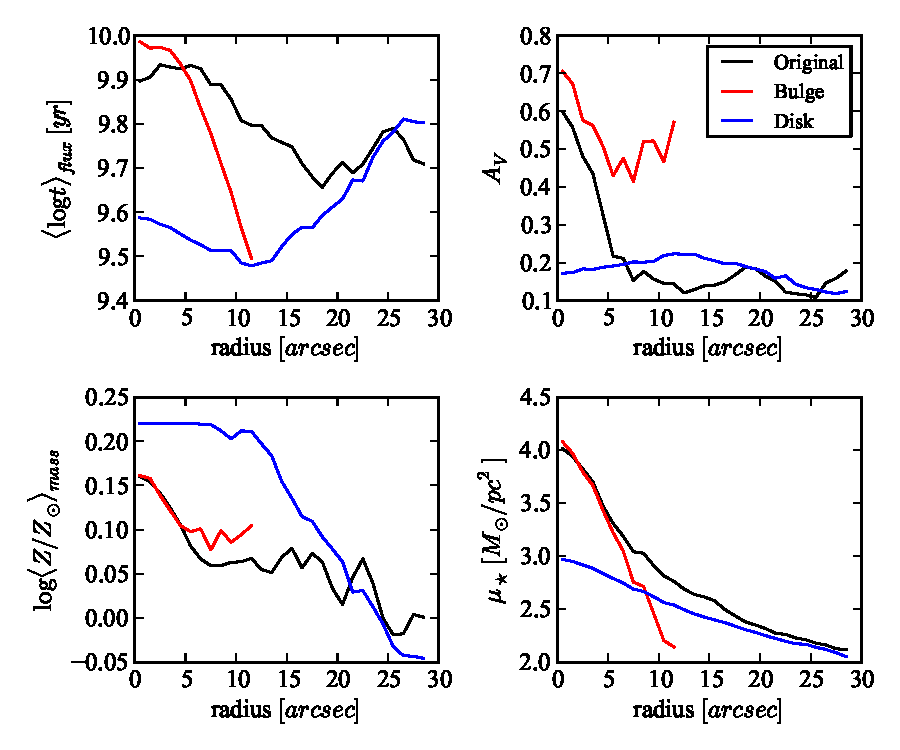
\includegraphics{figuras/decomp-at-aZ-AV-mu}
	\caption[Perfil radial das propriedades do bojo, disco, e total] {Perfil
	radial das propriedades físicas do bojo (vermelho), disco (azul), e original
	(preto). (cima, esquerda) Idade estelar média ponderada pela luminosidade.
	(baixo, esquerda) Metalicidade estelar média ponderada pela massa estelar.
	(cima, direita) Atenuação por poeira, na banda $V$. (baixo, direita) Desidade
	superficial de massa estelar. O Bojo vai somente até $12"$, que corresponde a
	$3\,R_{50}$.}
	\label{fig:decompSynRadprof}
\end{figure}

\begin{figure}
	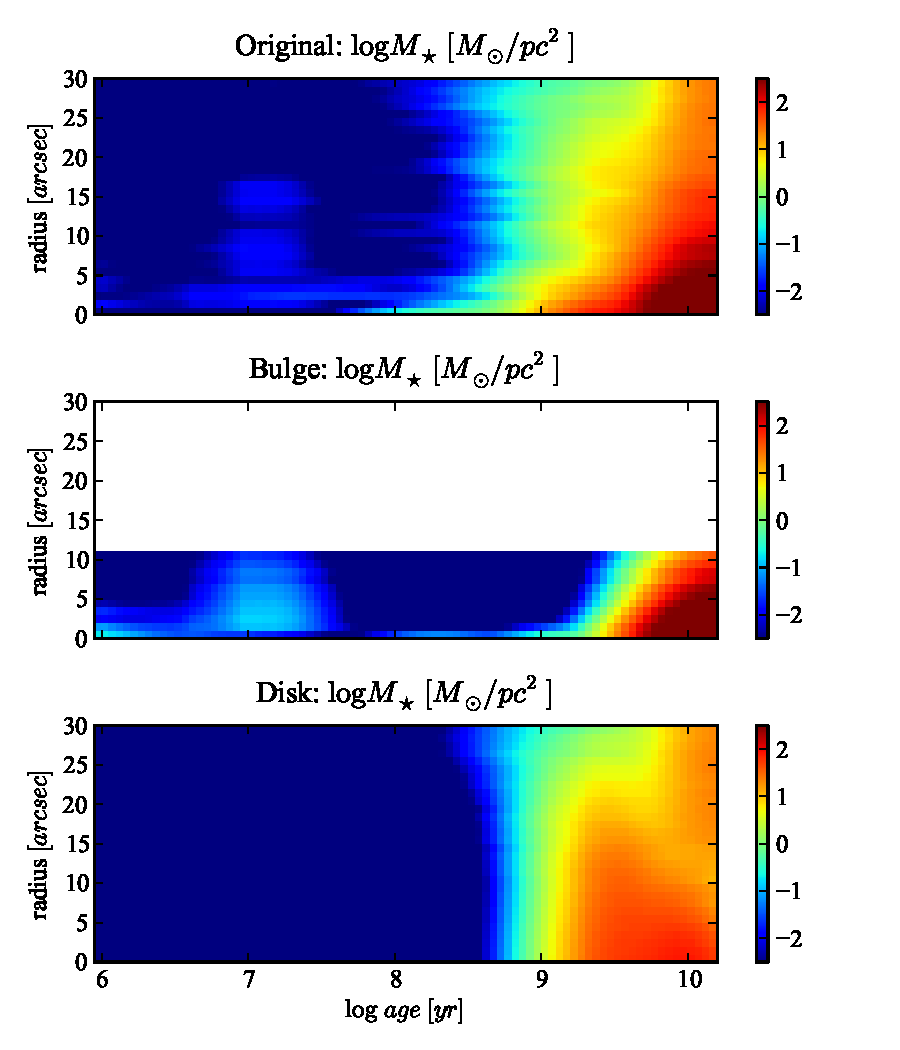
\includegraphics{figuras/decomp-sfh}
	\caption[Histórico de formação estelar do bojo, disco, e total] {Histórico de
	formação estelar da galáxia original (cima), bojo (meio) e disco (baixo). Os
	gráficos mostram quanta massa por unidade de área foi transformada em estrelas,
	em cada {\em bin} de raio e idade. O Bojo vai somente até $12"$, que
	corresponde a $3\,R_{50}$.}
	\label{fig:decompSynSfh}
\end{figure}

Através da decomposição morfológica realizada neste trabalho, foram obtidos
cubos de síntese espectral para o bojo e o disco de uma galáxia. As propriedades
físicas destas componentes são a grosso modo compatíveis com o que se espera de
um bojo e um disco. É preciso levar em conta, entretanto, que estes são resultados
preliminares. Testes similares aos apresentados anteriormente, com simulações de
galáxias com histórico de formação estelar mais realistas são fundamentais para
determinar a confiabilidade do método.

% End of this chapter
